
\section{Models}\label{sec:models}
In this section, we first describe the basic encoder-decoder RNN that serves as our baseline and then propose several novel models for summarization, each addressing a specific weakness in the baseline.

\subsection{Encoder-Decoder RNN with Attention and Large Vocabulary Trick}\label{sec:enc_dec}
Our baseline model corresponds to the neural machine translation model used in \newcite{nmt}. The encoder consists of a bidirectional GRU-RNN \cite{gru_rnn}, while the decoder consists of a uni-directional GRU-RNN with the same hidden-state size as that of the encoder, and an attention mechanism over the source-hidden states and a soft-max layer over target vocabulary to generate words. In the interest of space, we refer the reader to the original paper for a detailed treatment of this model.
%\subsection{Large Vocabulary Trick}\label{sec:lvt}
In addition to the basic model, we also adapted to the summarization problem, the large vocabulary `trick' (LVT) described in \newcite{lvt}. In our approach, the decoder-vocabulary of each mini-batch is restricted to words in the source documents of that batch. In addition, the most frequent words in the target dictionary are added until the vocabulary reaches a fixed size. %We call this the LVT-vocabulary.
The aim of this technique is to reduce the size of the soft-max layer of the decoder which is the main computational bottleneck. In addition, this technique also speeds up convergence by focusing the modeling effort only on the words that are essential to a given example. This technique is particularly well suited to summarization since a large proportion of the words in the summary come from the source document in any case.

%\subsection{Vocabulary expansion}\label{sec:expand}
%LVT addresses the computational bottleneck of a large softmax layer, but at the same time, it sacrifices some of its ability to produce novel but meaningful words, as it now relies heavily on the source vocabulary. To overcome this shortcoming, we propose to expand the LVT vocabulary by adding the 1-nearest-neighbors of all words in the source document, as measured by cosine similarity in the word embeddings space. We hope this technique will help achieve balance between the mutually conflicting goals of a more focused model vs. better generalizability.

\subsection{Capturing Keywords using Feature-rich Encoder}\label{sec:feats}
In summarization, one of the key challenges is to identify the key concepts and key entities in the document, around which the story revolves. In order to accomplish this goal, we may need to go beyond the word-embeddings-based representation of the input document and capture additional linguistic features such as parts-of-speech tags, named-entity tags, and TF and IDF statistics of the words. We therefore create additional look-up based embedding matrices for the vocabulary of each tag-type, similar to the embeddings for words. For continuous features such as TF and IDF, we convert them into categorical values by discretizing them into a fixed number of bins, and use one-hot representations to indicate the bin number they fall into. This allows us to map them into an embeddings matrix like any other tag-type. Finally, for each word in the source document, we simply look-up its embeddings from all of its associated tags and concatenate them into a single long vector, as shown in Fig. \ref{fig:feature_rich_encoder}.  %This will replace the word-based-embeddings in the original model. 
On the target side, we continue to use only word-based embeddings as the representation.

\begin{figure}[ht]
    \vspace{-0.3in}
	\centering
  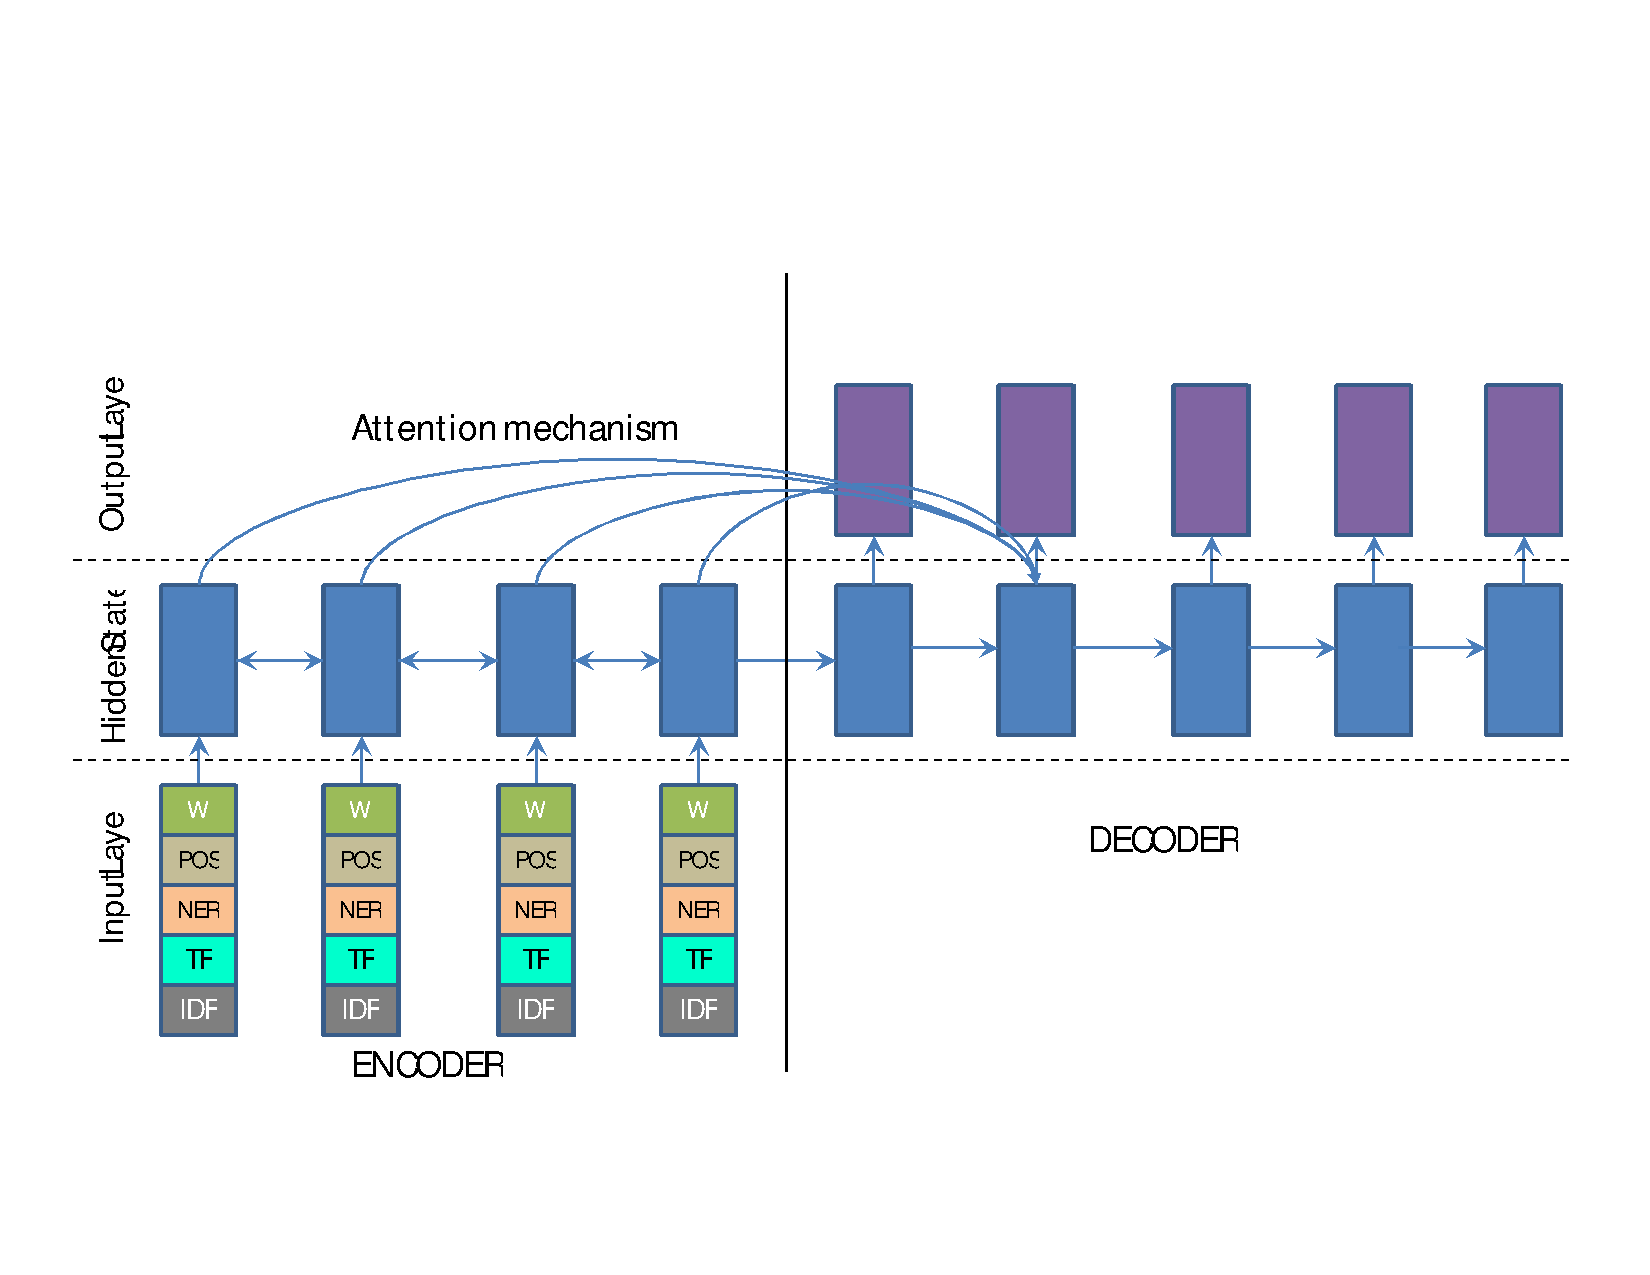
\includegraphics[width=0.5\textwidth]{feature_rich_encoder.PDF}
  \vspace{-0.6in}
	\caption{{\small Feature-rich-encoder: We use one embedding vector each for POS, NER tags and discretized TF and IDF values, which are concatenated together with word-based embeddings as input to the encoder.}}
	\label{fig:feature_rich_encoder}
\end{figure}

\subsection{Modeling Rare/Unseen Words using Switching Generator-Pointer}\label{sec:switch}
Often-times in summarization, the keywords or named-entities in a test document that are central to the summary may actually be unseen or rare with respect to training data. Since the vocabulary of the decoder is fixed at training time, it cannot emit these unseen words. Instead, a most common way of handling these out-of-vocabulary (OOV) words is to emit  an `UNK' token as a placeholder. However this does not result in legible summaries. In summarization, an intuitive way to handle such OOV words is to simply point to their location in the source document instead. We model this notion using our novel switching decoder/pointer architecture which is graphically represented in Figure \ref{fig:switching_generator_pointer}. In this model, the decoder is equipped with a `switch' that decides between using the generator or a pointer at every time-step. If the switch is turned on, the decoder produces a word from its target vocabulary in the normal fashion. However, if the switch is turned off, the decoder instead generates a pointer to one of the word-positions in the source. The word at the pointer-location is then copied into the summary.  The switch is modeled as a sigmoid activation function over a linear layer based on the entire available context at each time-step as shown below.
% hidden state of the decoder, embedding vector from previous emission and context vector, as shown below:
\begin{eqnarray}
P(s_i=1) &=& \sigma({{\bf v}^s}\cdot({\bf W}^s_h{\bf h}_i + {\bf W}^s_e{\bf E}[o_{i-1}] \nonumber\\
             &+& {\bf W}^s_c{\bf c}_i + {\bf b}^s)),\nonumber
\end{eqnarray}
where $P(s_i=1)$ is the probability of the switch turning on at the $i^{th}$ time-step of the decoder, ${\bf h}_i$ is the hidden state,  ${\bf E}[o_{i-1}]$ is the embedding vector of the emission from the previous time step, ${\bf c_i}$ is the attention-weighted context vector, and ${\bf W}_h^s, {\bf W}_e^s, {\bf W}_c^s, {\bf b}^s$ and ${\bf v}^s$ are the switch parameters. We use attention distribution over word positions in the document as the distribution to sample the pointer from.
\begin{eqnarray}
P^a_i(j)    &\propto&  \exp({{\bf v}^a}\cdot({\bf W}_h^a{\bf h}_{i-1} + {\bf W}^a_e{\bf E}[o_{i-1}] \nonumber\\
            &+& {\bf W}^a_c{\bf h}^d_j + {\bf b}^a)), \nonumber \\
 p_i &=& \arg\max_j (P^a_i(j))~\mbox{for}~j \in \{1,\ldots,N_d\}\nonumber.
\end{eqnarray}
In the above equation, $p_i$ is the pointer value at $i^{th}$ word-position in the summary, sampled from the attention distribution ${\bf P}^a_i$ over the document word-positions $j \in \{1,\ldots,N_d\}$, where $P^a_i(j)$ is the probability of the $i^{th}$ time-step in the decoder pointing to the $j^{th}$ position in the document, and ${\bf h}^d_j$ is the encoder's hidden state at position $j$. %, is parameterized as shown above, in terms of the decoder's previous hidden state ${\bf h}_{i-1}$, previous emission $o_{i-1}$, and the encoder's concatenated hidden state ${\bf h}_j$.

At training time, we provide the model with explicit pointer information whenever the summary word does not exist in the target vocabulary. When the OOV word in summary occurs in multiple document positions, we break the tie in favor of its first occurrence. At training time, we optimize the conditional log-likelihood shown below, with additional regularization penalties.
\begin{eqnarray}
&& \log P({\bf y}|{\bf x}) = \sum_i (g_i\log \{P(y_i | {\bf y}_{-i}, {\bf x})P(s_i)\} \nonumber\\
 &&+  (1-g_i)\log\{P(p(i)|{\bf y}_{-i},{\bf x})(1-P(s_i))\})\nonumber
\end{eqnarray}
where ${\bf y}$ and ${\bf x}$ are the summary and document words respectively, $g_i$ is an indicator function that is set to 0 whenever the word at position $i$ in the summary is OOV with respect to the decoder vocabulary. At test time, the model decides automatically at each time-step whether to generate or to point, based on the estimated switch probability $P(s_i)$.  We simply use the $\arg\max $ of the posterior probability of generation or pointing to generate the best output at each time step.

The pointer mechanism may be more robust in handling rare words because it uses the encoder's hidden-state representation of rare words to decide which word from the document to point to. Since the hidden state depends on the entire context of the word, the model is able to accurately point to unseen words although they do not appear in the target vocabulary.\footnote{Even when the word does not exist in the source vocabulary, the pointer model may still be able to identify the correct position of the word in the source since it takes into account the contextual representation of the corresponding 'UNK' token encoded by the RNN. Once the position is known, the corresponding token from the source document can be displayed in the summary even when it is not part of the training vocabulary either on the source side or the target side.}  %Given a large number of training examples, the switch learns to pick the pointer over generator for production of rare words.
%For a more detailed description of this model and experiments on multiple problems, please refer to the parallel work published by some of the co-authors of this paper \cite{caglar_pointernet}. 
%\ramesh{Need to restructure this paragraph after reading Luong's paper. Also add an anonymous citation to Caglar's paper}.


\begin{figure}[ht]
    \vspace{-0.3in}
	\centering
  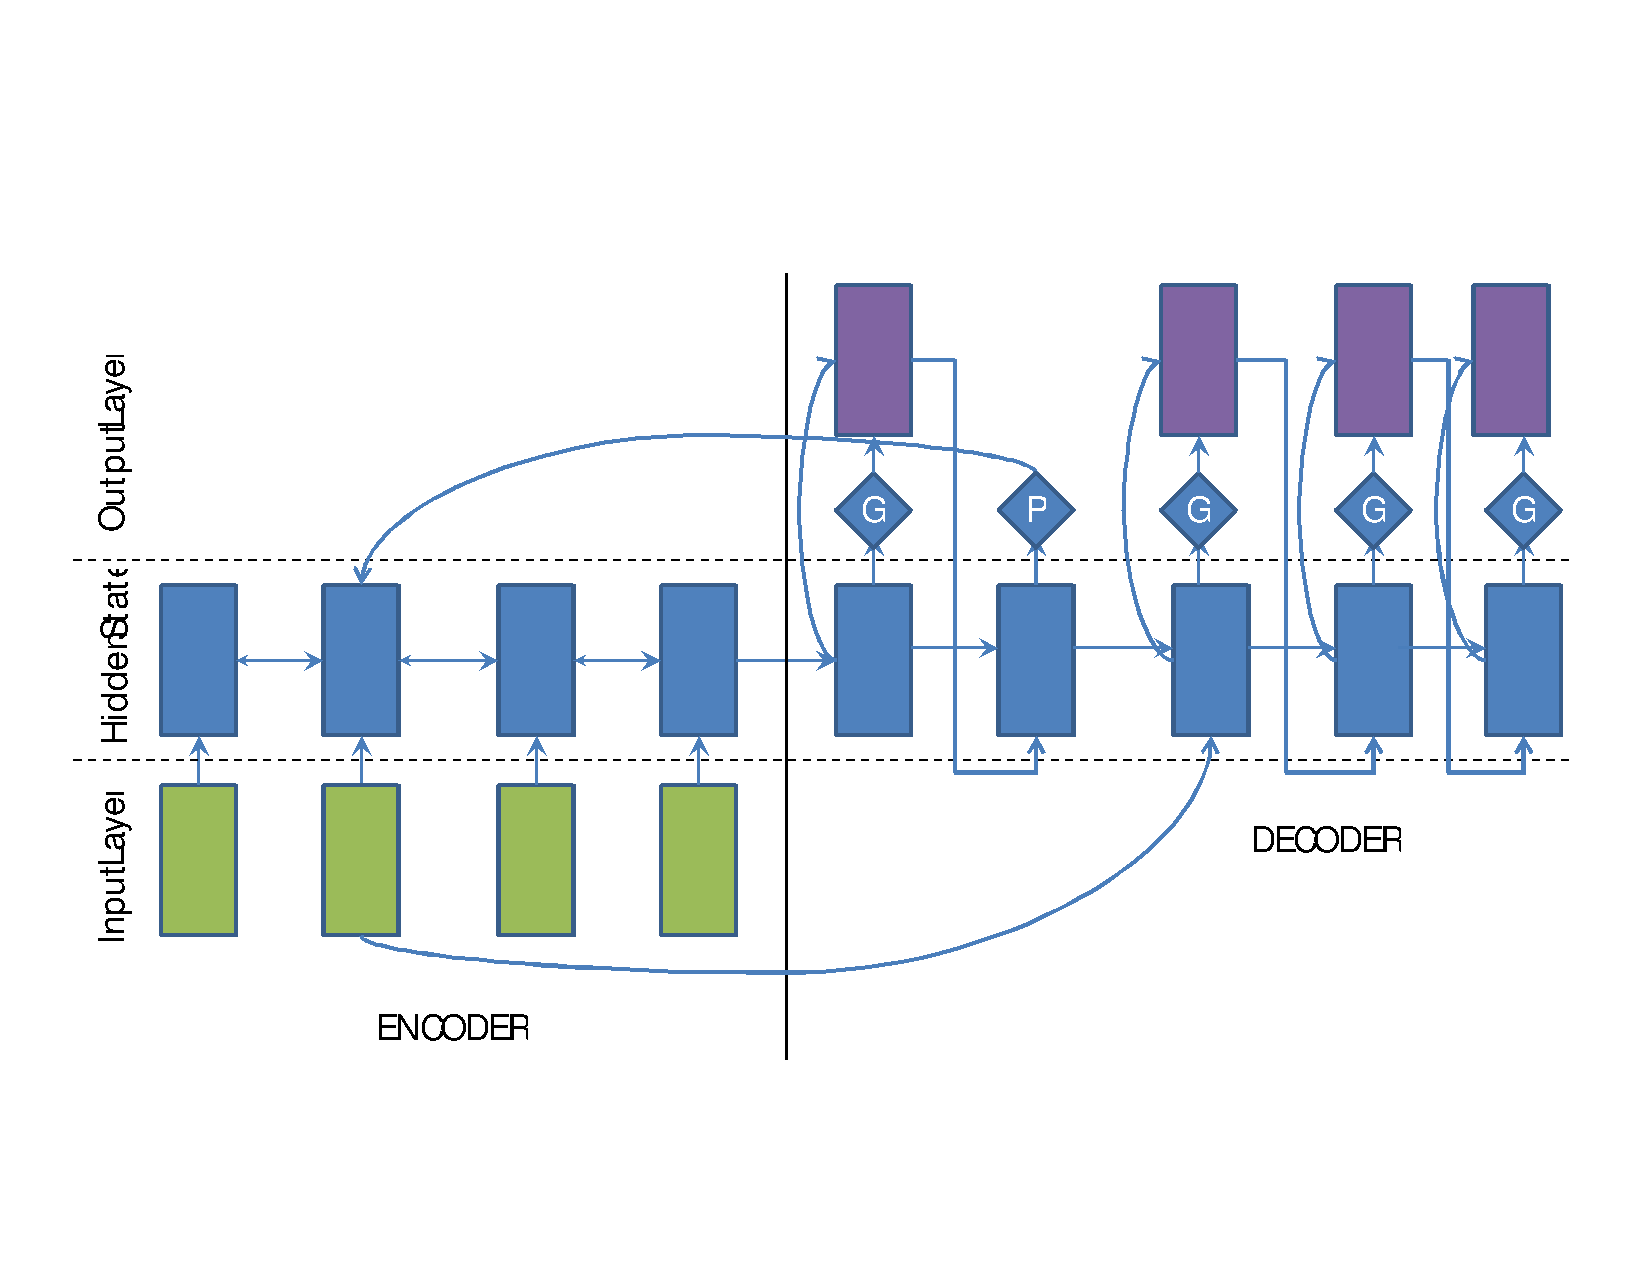
\includegraphics[width=0.5\textwidth]{switching_generator_pointer.PDF}
  \vspace{-0.6in}
	\caption{{\small Switching generator/pointer model: When the switch shows 'G', the traditional generator consisting of the softmax layer is used to produce a word, and when it shows 'P', the pointer network is activated to copy the word from one of the source document positions. When the pointer is activated, the embedding from the source is used as input for the next time-step as shown by the arrow from the encoder to the decoder at the bottom.}}
	\label{fig:switching_generator_pointer}
\end{figure}

\subsection{Capturing Hierarchical Document Structure with Hierarchical Attention}\label{sec:hierarchical}
In datasets where the source document is very long, in addition to identifying the keywords in the document, it is also important to identify the key sentences from which the summary can be drawn. This model aims to capture this notion of two levels of importance using two bi-directional RNNs on the source side, one at the word level and the other at the sentence level. The attention mechanism operates at both levels simultaneously. The word-level attention is further re-weighted by the corresponding sentence-level attention and re-normalized as shown below:
\begin{eqnarray}
P^a(j) &=&  \frac{P^a_w(j)P^a_s(s(j))}{\sum_{k=1}^{N_d} P^a_w(k)P^a_s(s(k))},\nonumber
\end{eqnarray}
where $P^a_w(j)$ is the word-level attention weight at $j^{th}$ position of the source document, and $s(j)$ is the ID of the sentence at $j^{th}$ word position, $P^a_s(l)$ is the sentence-level attention weight for the $l^{th}$ sentence in the source, $N_d$ is the number of words in the source document, and $P^a(j)$ is the re-scaled attention at the  $j^{th}$ word position. The re-scaled attention is then used to compute the attention-weighted context vector that goes as input to the hidden state of the decoder. Further, we also concatenate additional positional embeddings to the hidden state of the sentence-level RNN to model positional importance of sentences in the document. This architecture therefore models key sentences as well as keywords within those sentences jointly. A graphical representation of this model is displayed in Figure \ref{fig:hierarchical_attention}. 

\begin{figure}[ht]
    \vspace{-0.3in}
	\centering
  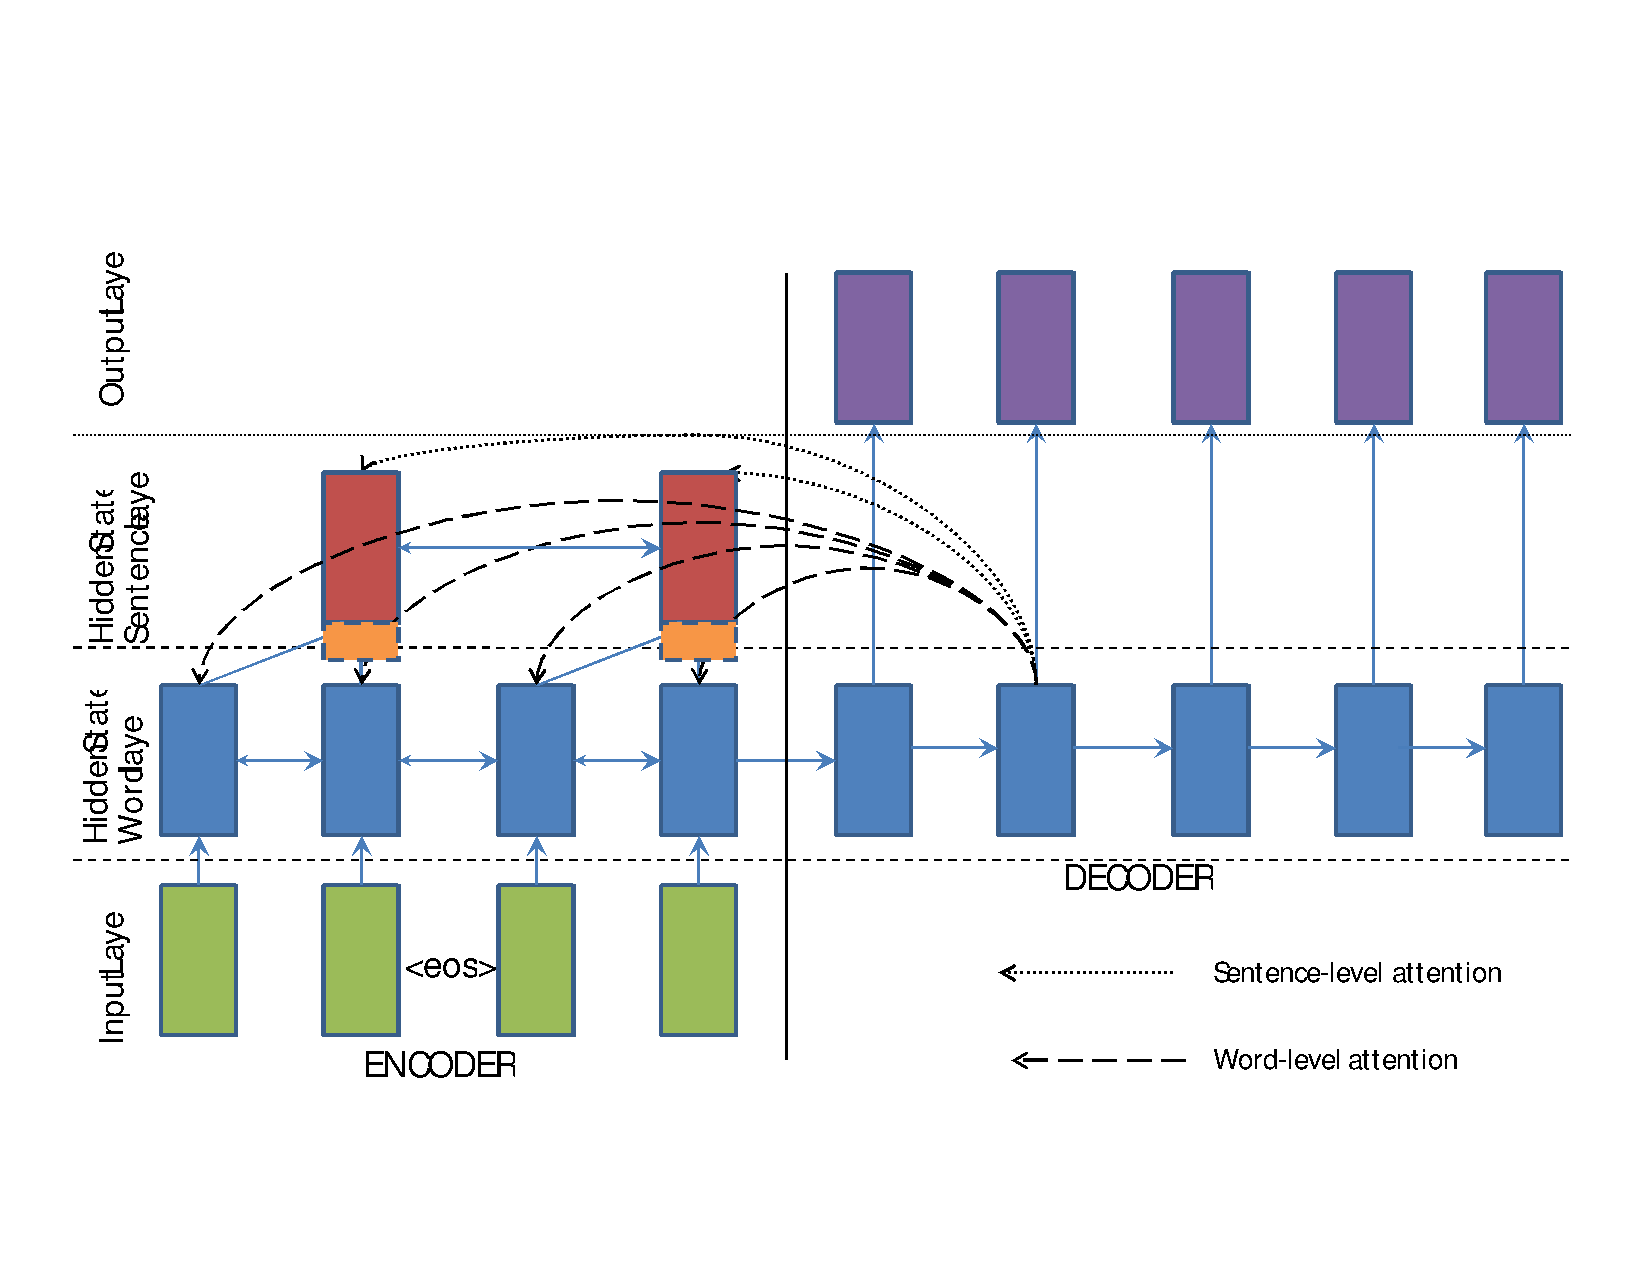
\includegraphics[width=0.5\textwidth]{hierarchical_attention.PDF}
  	\vspace{-0.6in}
	\caption{{\small Hierarchical encoder with hierarchical attention: the attention weights at the word level, represented by the dashed arrows are re-scaled by the corresponding sentence-level attention weights, represented by the dotted arrows. The dashed boxes at the bottom of the top layer RNN represent sentence-level positional embeddings concatenated to the corresponding hidden states.}}
	\label{fig:hierarchical_attention}
\end{figure}

%This model is still producing repeated words. Need to rethink the model. Omitting for acl. --Ramesh.
%\subsection{Decoder with Memory}\label{sec:memory}
%Although RNNs are expected to model long-distance dependencies between words in a sequence, in practice, they tend to forget their history beyond a few time-steps due to the compressed representation of the hidden state \cite{lstmn}. This may result in the decoder repeating the same set of words, phrases or even sentences in the summary. To mitigate this problem, we propose a simple extension to the decoder, wherein, we maintain a running average of the hidden states of the decoder until the current time-step and provide this as an additional input to the computation of the new hidden state. We input this information as an additional linear layer after the application of the update-gate in the GRU followed by a {\it tanh} activation function, to force the model to `memorize' a foot-print of its past history. 



